\section{Evaluation}

\subsection{Execution Time}
Figure ~\ref{Fig:buildmodel} shows the time for building the model with different algorithms under different minimum supports. We can see that with the minimum support increasing, the time for building the model is decreased in three algorithms, which makes sense since the greater the minimum support is, the less rules are left.

\begin{figure}
\centering
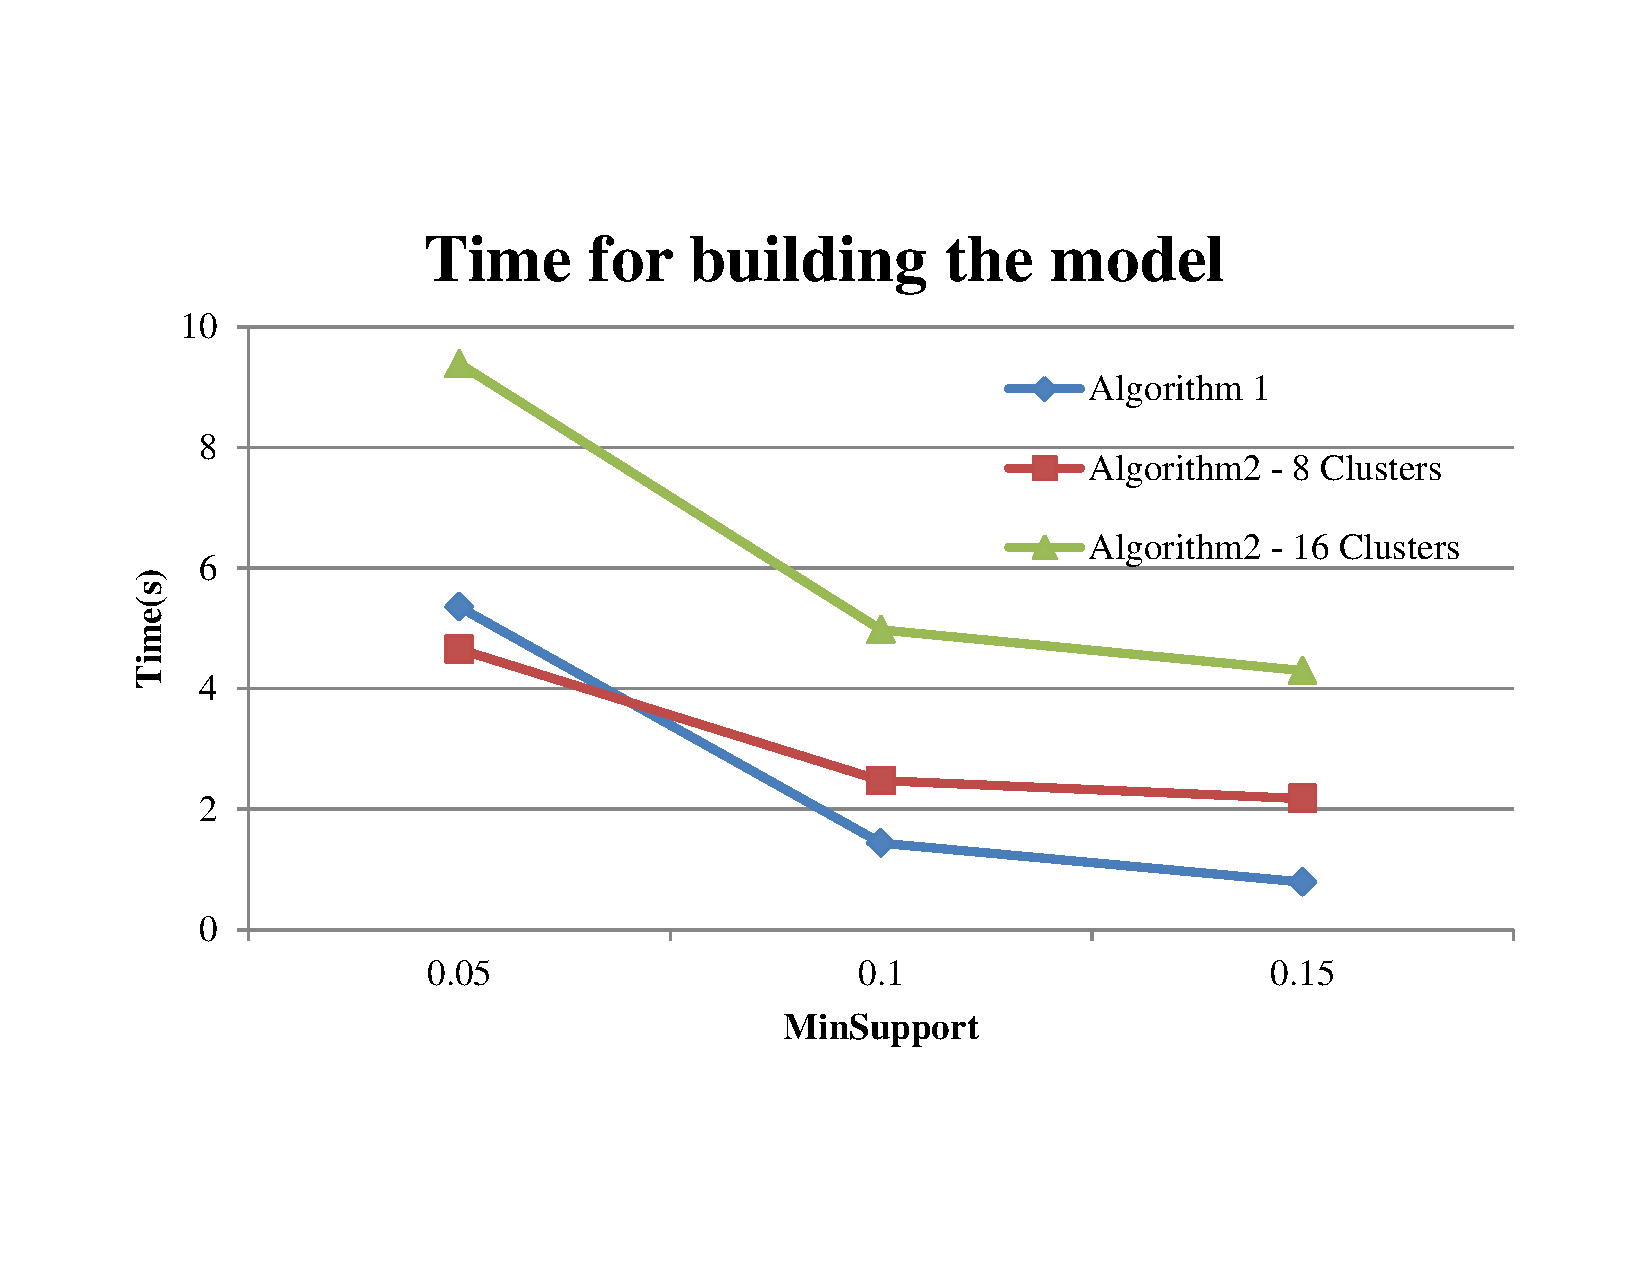
\includegraphics[width=0.8\textwidth]{buildmodel}
\caption{\footnotesize Time to build the model, i.e. to generate association
rules, for the two algorithms with different minimum supports. (We don't include the clustering time in Algorithm 2)}
\label{Fig:buildmodel}
\end{figure}

The time for testing the model with Algorithm 1 is shown in Figure ~\ref{Fig:TestTime1}. We can see that under the same minimum support, with K increasing, the time for building the model is increased, since we need to check more rules to predict the topics of the document. The time for testing the model with Algorithm 2 is shown in Figure ~\ref{Fig:TestTime2}. With different Ks, the testing time doesn't changed a lot since determining the nearest cluster accounts for a large amount of testing time. This is why Algorithm 2 with 16 clusters takes more testing time than 8 clusters, and we don't compare the testing time between Algorithm 1 with Algorithm 2.

\begin{figure}
\centering
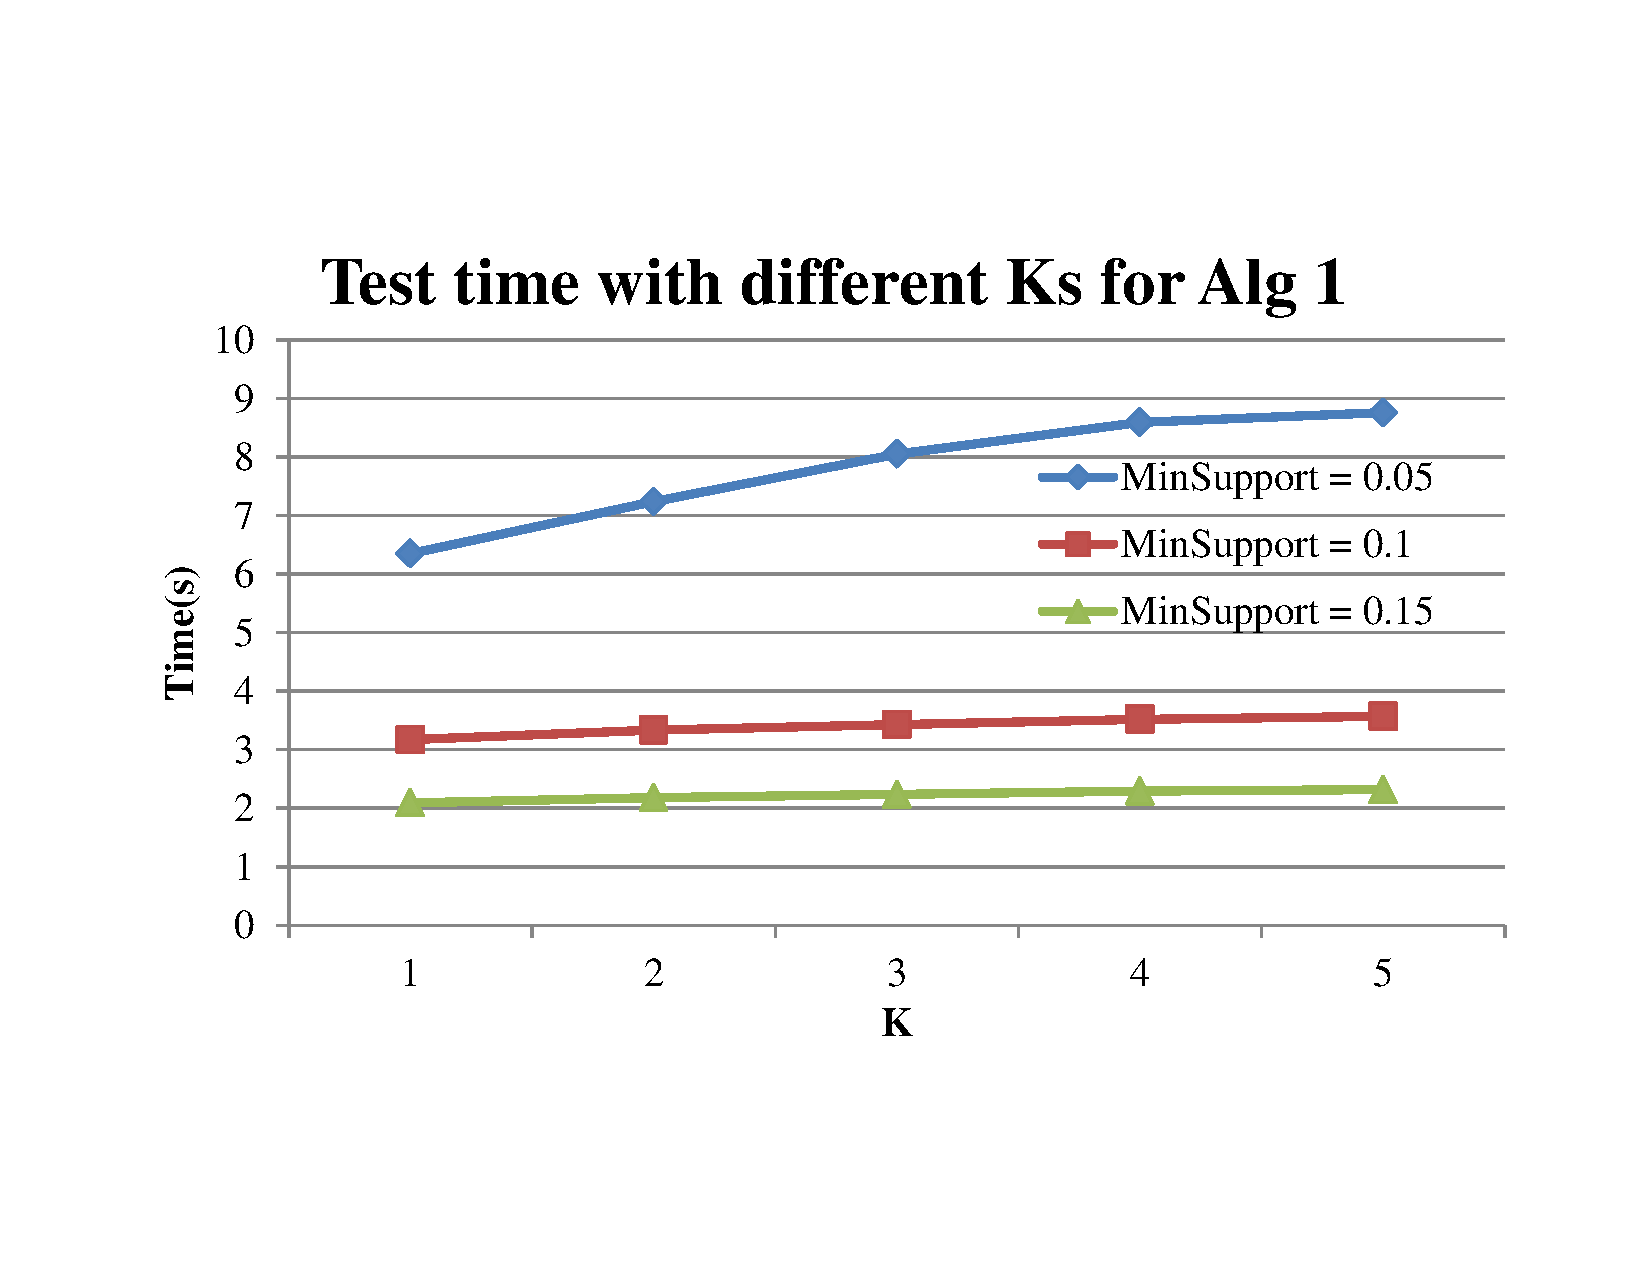
\includegraphics[width=0.8\textwidth]{TestingTime1}
\caption{\footnotesize Time to run the model over the test data, for algorithm
1 with different minimum supports and K values. }
\label{Fig:TestTime1}
\end{figure}

\begin{figure}
\centering
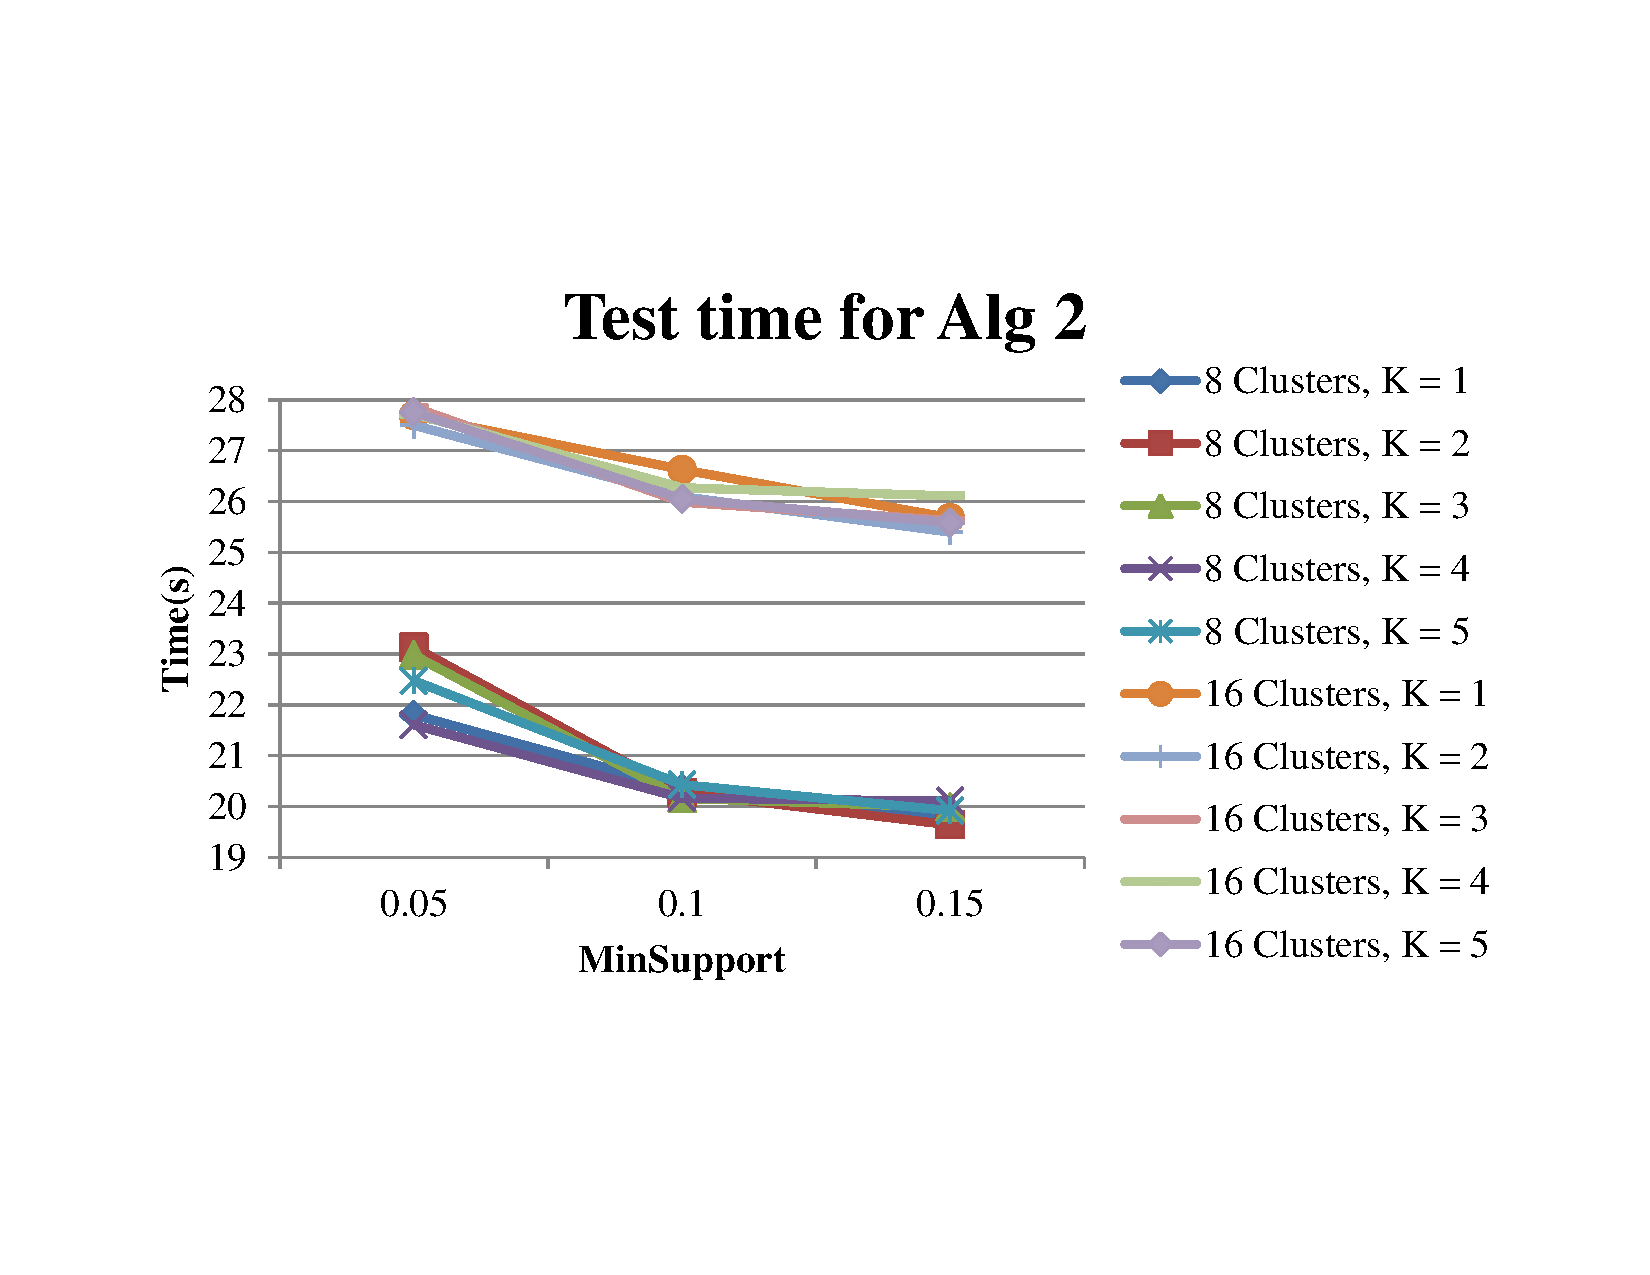
\includegraphics[width=0.8\textwidth]{TestingTime2}
\caption{\footnotesize Time to run the model over the test data, for algorithm
2 with different minimum supports and K values. }
\label{Fig:TestTime2}
\end{figure}

\subsection{Quality}
\subsubsection{Accuracy}
Except the Algorithm 1 with minimum support 0.05, Algorithm 2 is better than Algorithm 1 with the same parameters. And the accuracy of 16 clusters are better than that of 8 clusters. We notes that with K increasing, the accuracy is increased since more rules are used, more topics are predicted. According the accuracy we defined, the probility of the predicated topics overlapping with correct topics are increased.   

\begin{figure}
\centering
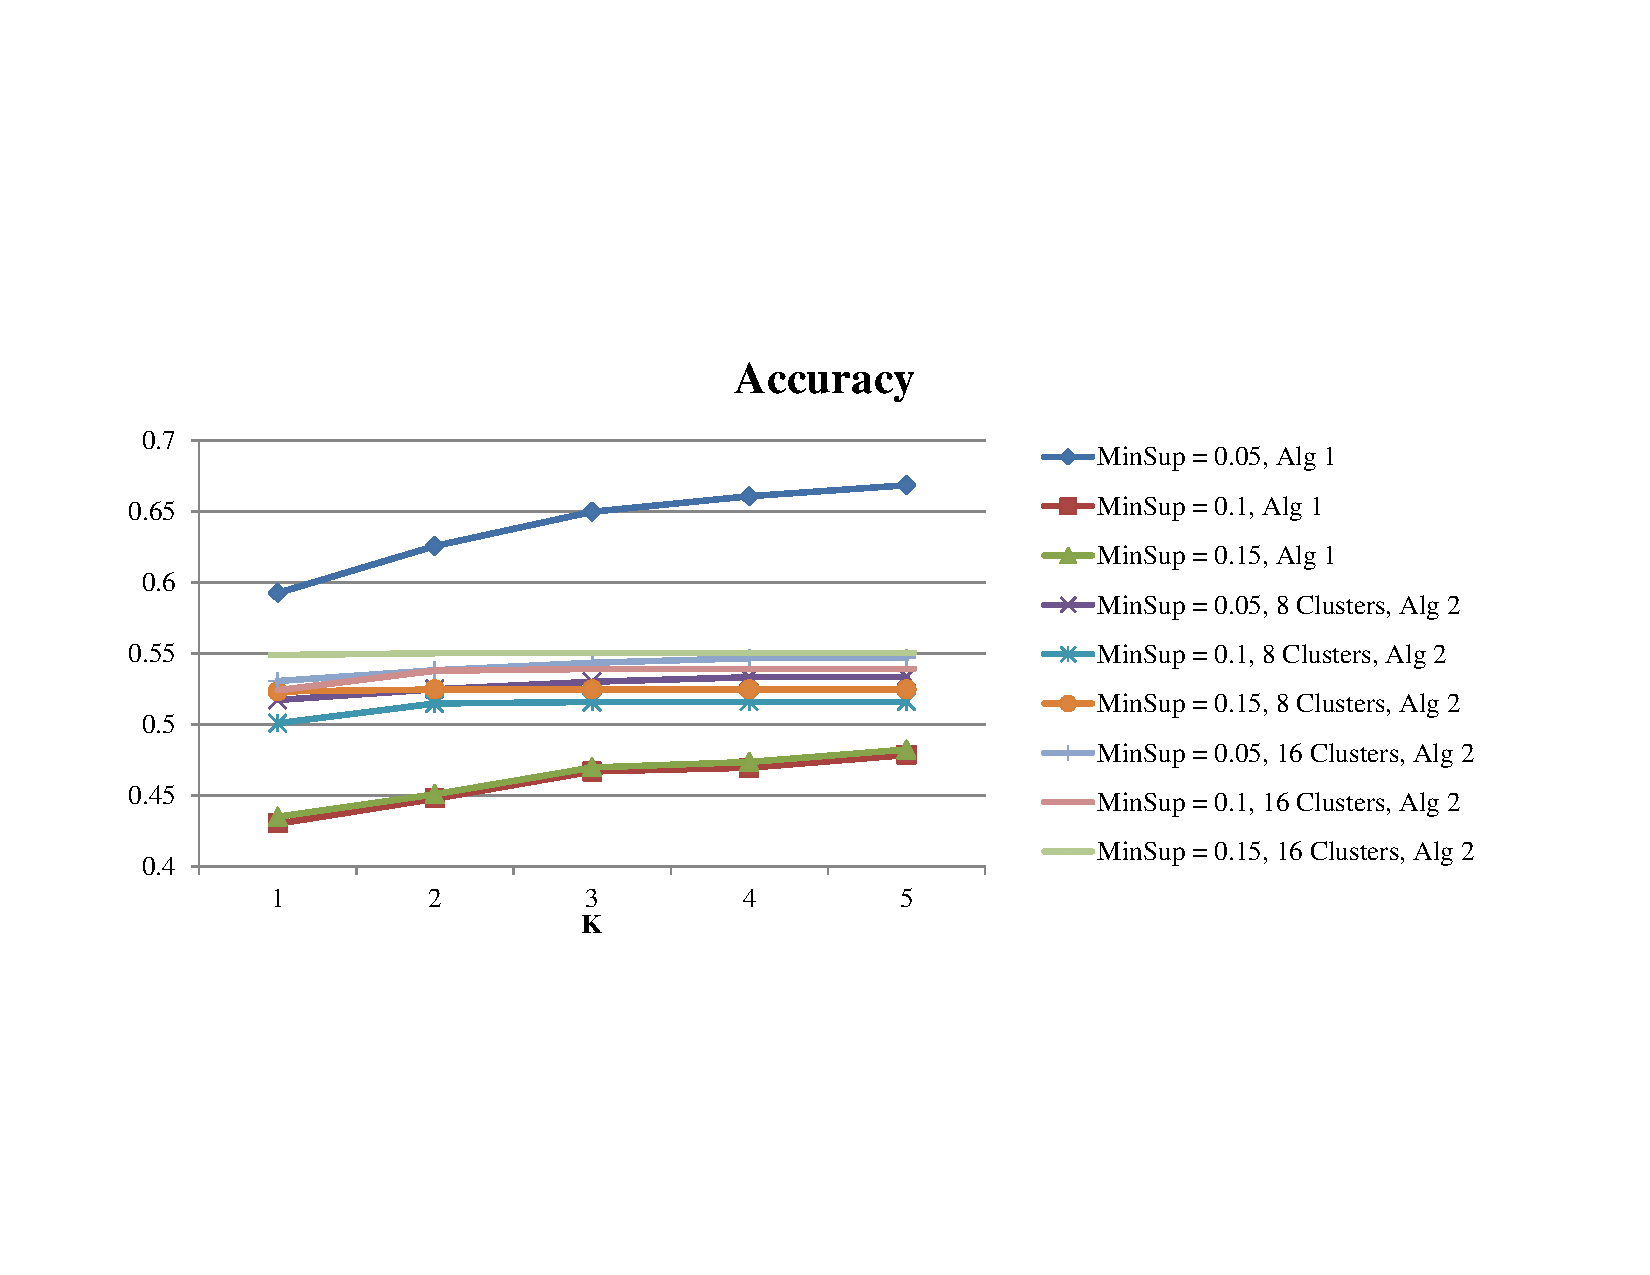
\includegraphics[width=0.8\textwidth]{Accuracy}
\caption{\footnotesize The accuracy for the two algorithms with different
parameters. }
\label{Fig:Accuracy}
\end{figure}

We can see from Figure ~\ref{Fig:F-measure} that F-measure(Alg 1) > F-measure(Alg 2, 8 clusters) > F-measure(Alg 2, 16 clusters) with different Ks and under different minimum support. The reason for this is that  the rules in the clusters are much less than the rules in the Algorithm 1, which results in less topics predicted, so the recall in Algorithm 2 is much smaller than Algorithm 1. And with the number of clusters increased, the situation is worse.
\subsubsection{F-measure}
\begin{figure*}
        \centering
        \begin{subfigure}[b]{0.3\textwidth}
         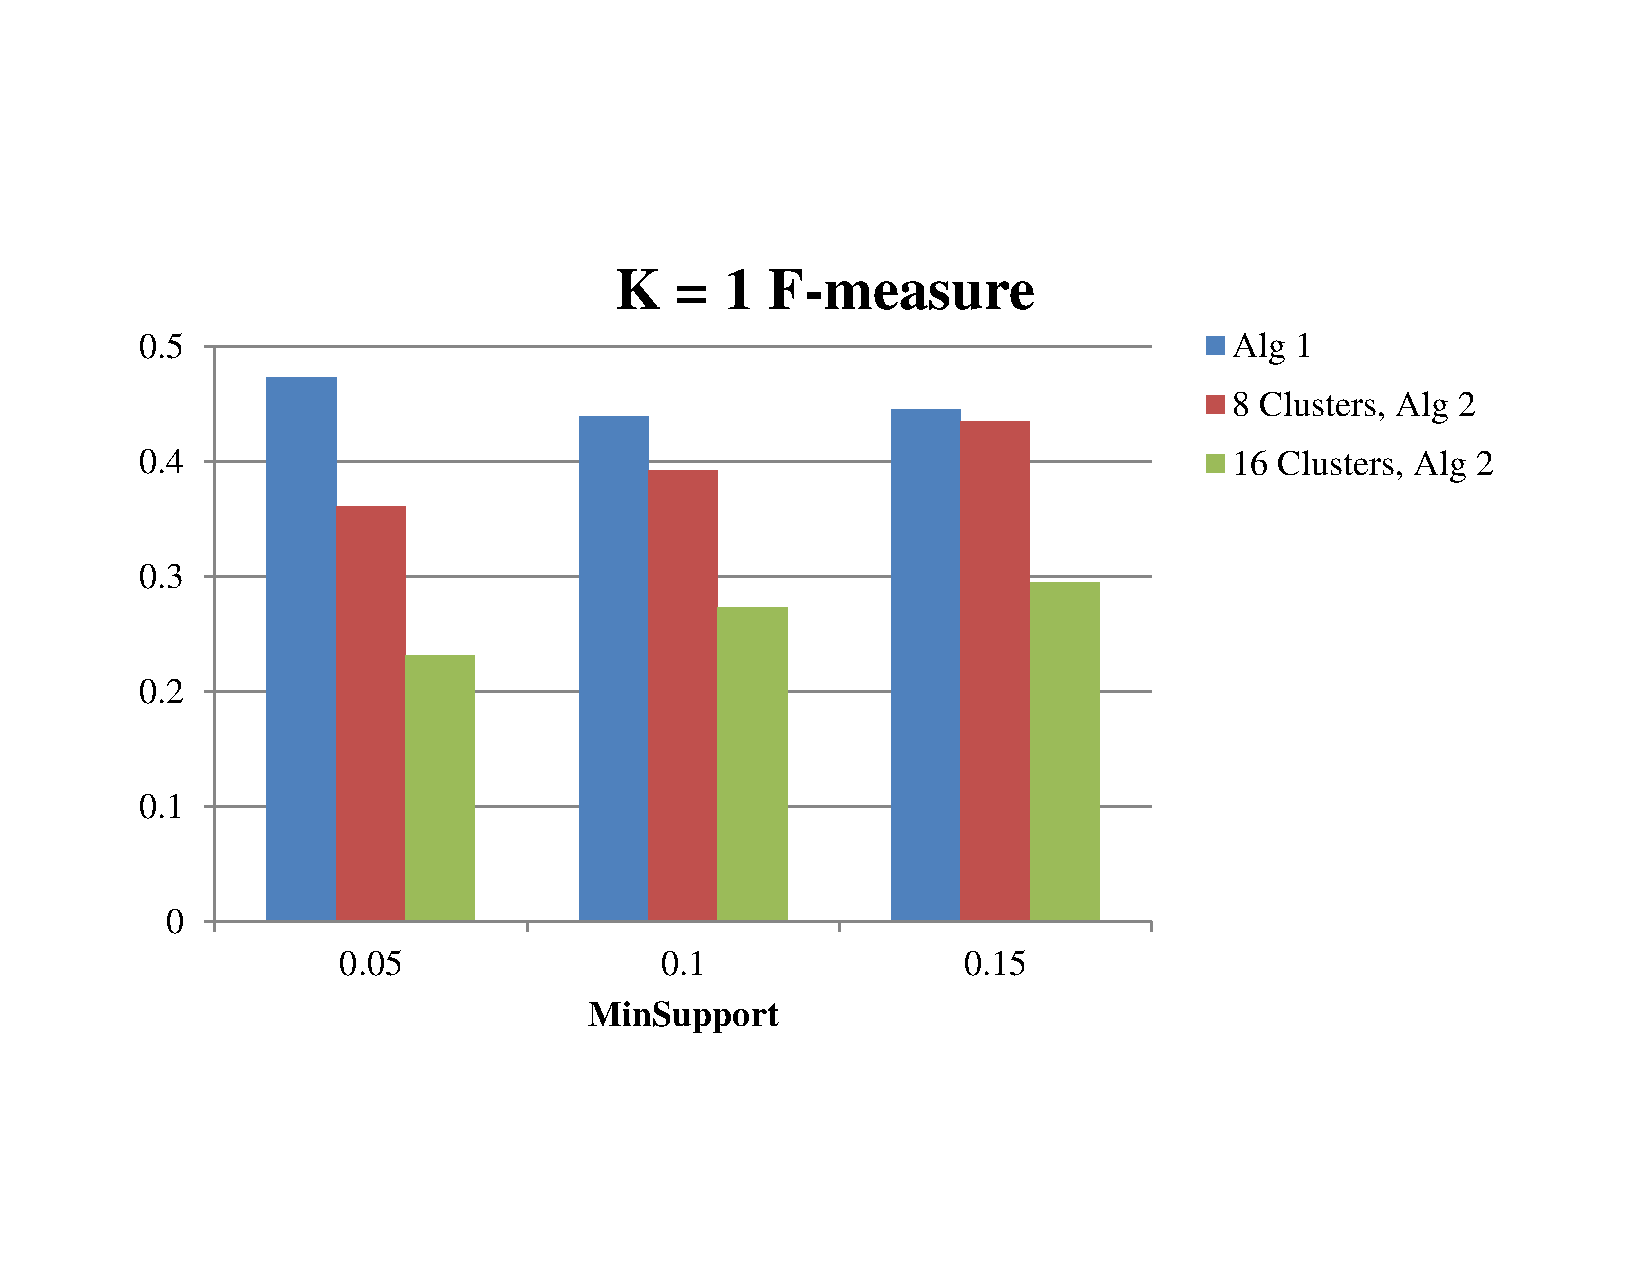
\includegraphics[width=\textwidth]{F-measure1}
         \caption{K = 1}
         \label{Fig:F-measure1}
        \end{subfigure}
        \begin{subfigure}[b]{0.3\textwidth}
         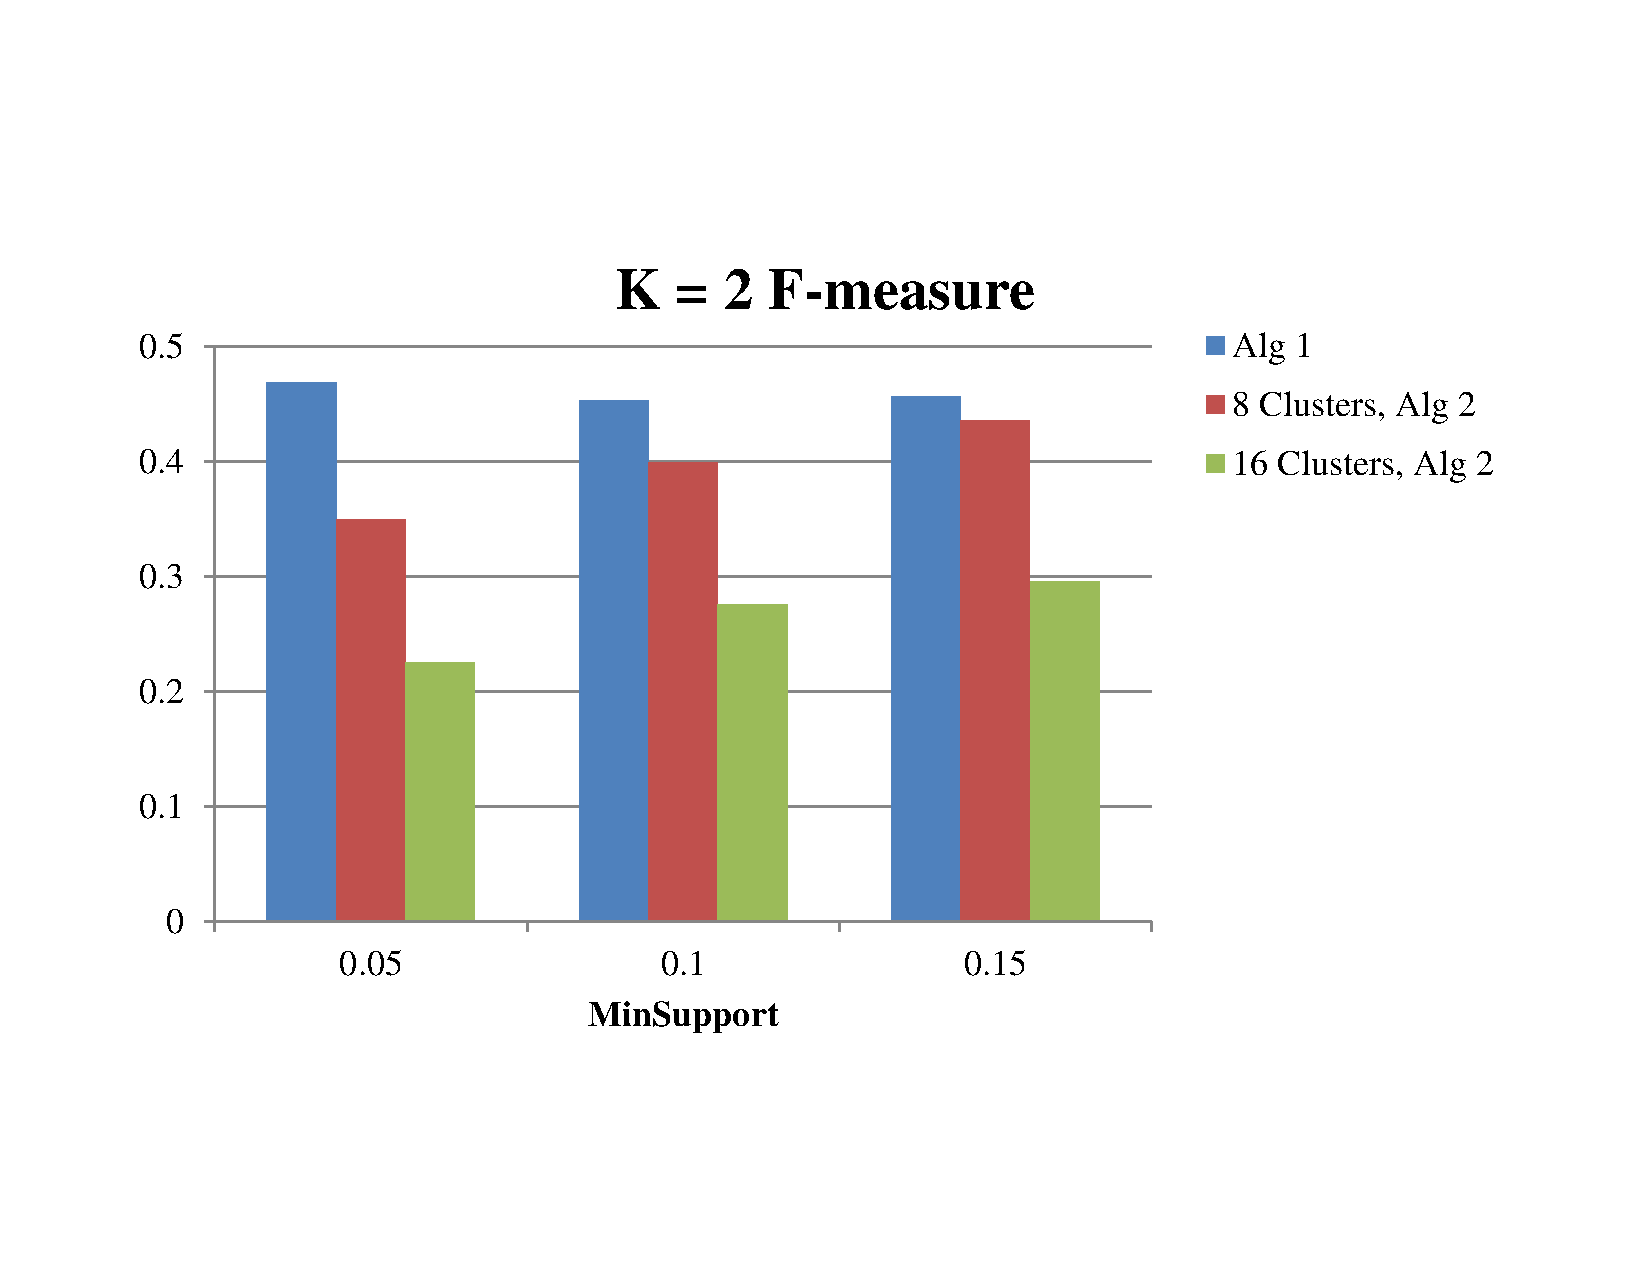
\includegraphics[width=\textwidth]{F-measure2}
         \caption{K = 2}
         \label{Fig:F-measure2}
        \end{subfigure}
        \begin{subfigure}[b]{0.3\textwidth}
         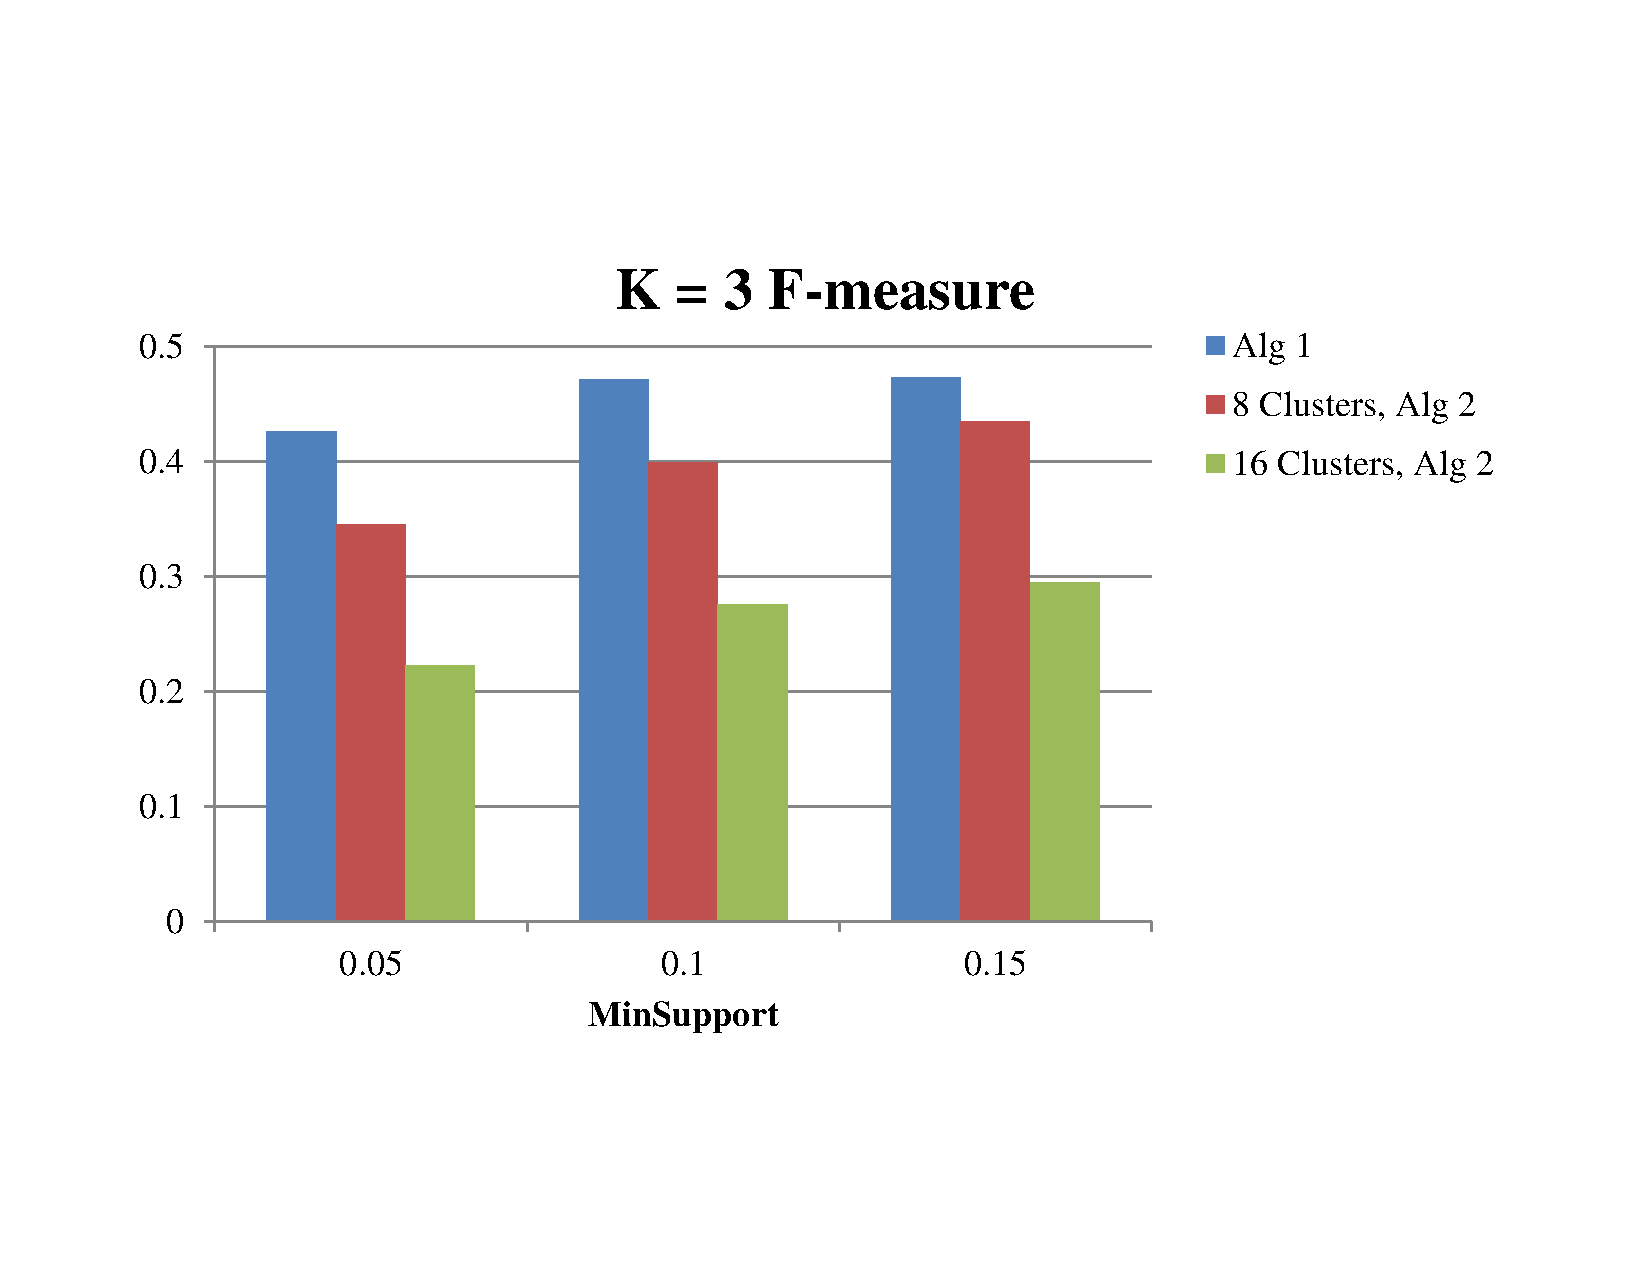
\includegraphics[width=\textwidth]{F-measure3}
         \caption{K = 3}
         \label{Fig:F-measure3}
        \end{subfigure}
        \begin{subfigure}[b]{0.3\textwidth}
         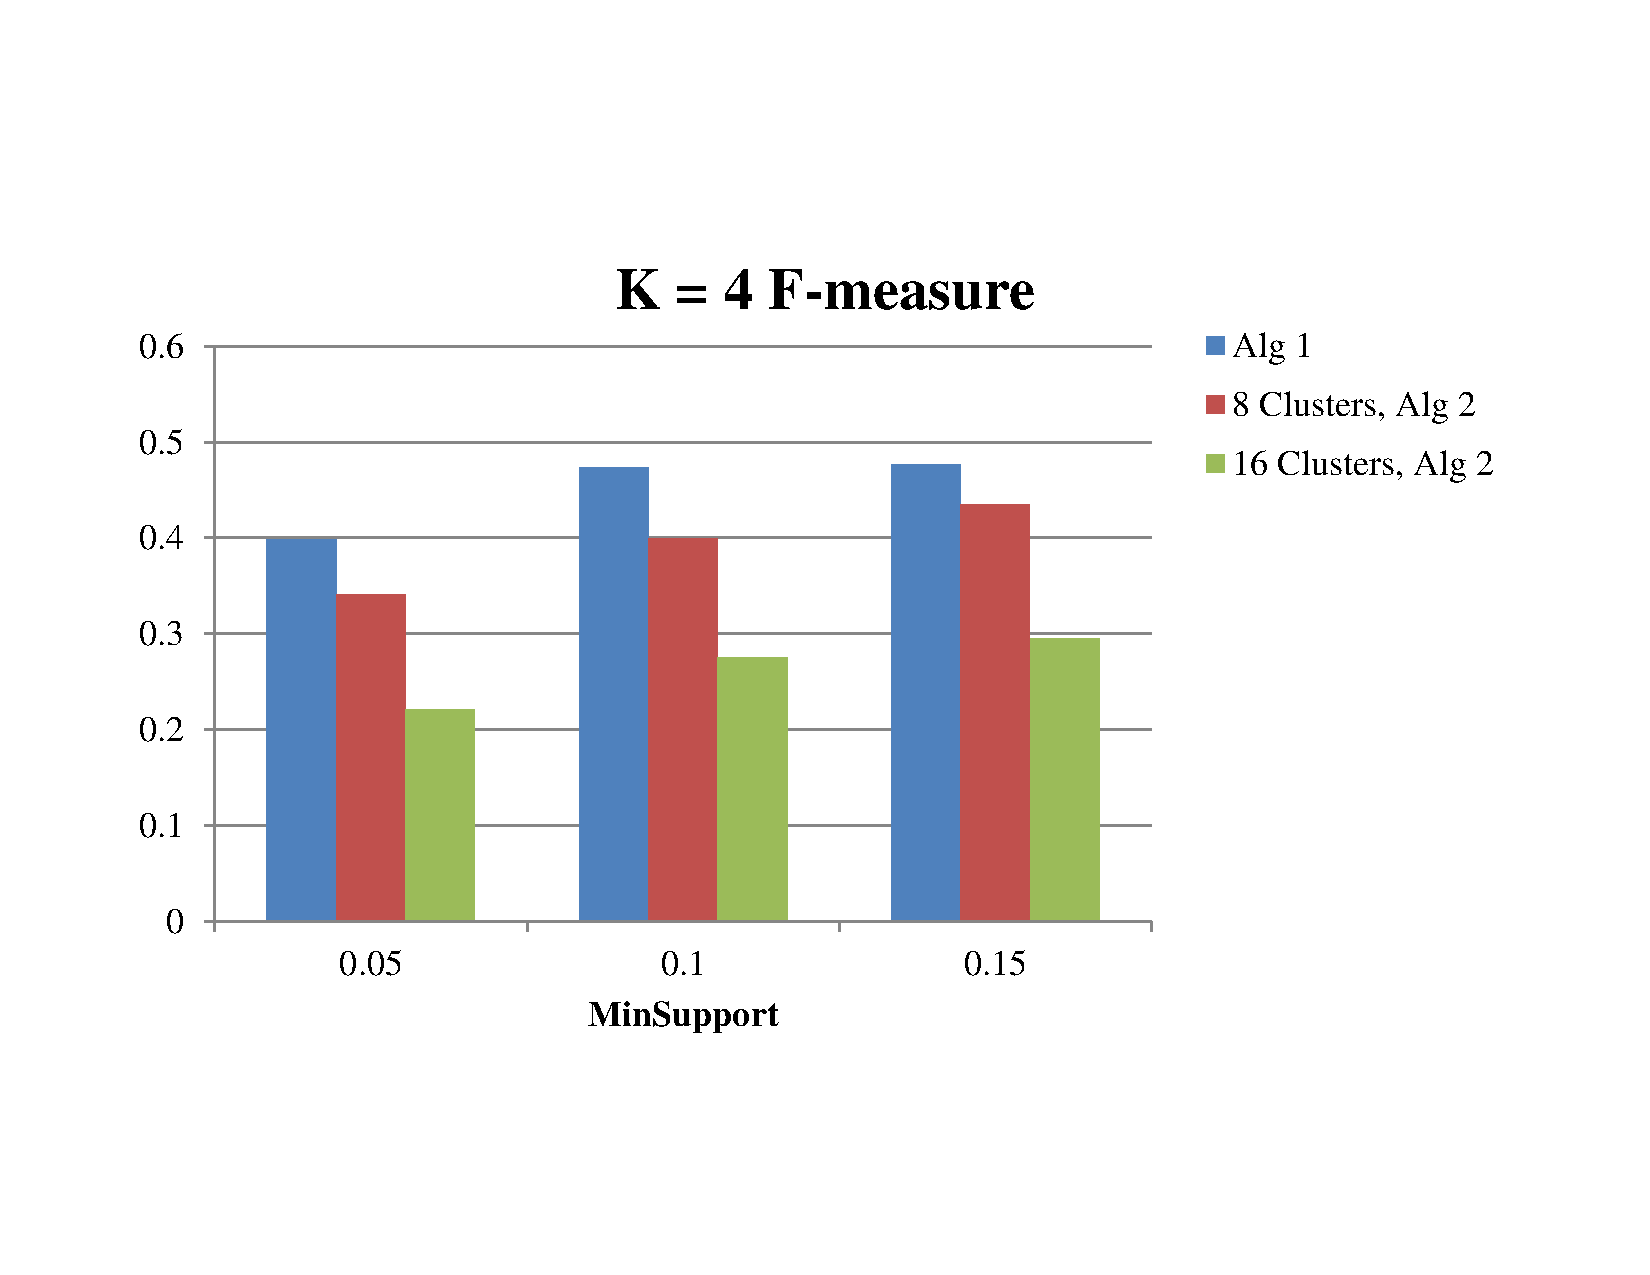
\includegraphics[width=\textwidth]{F-measure4}
         \caption{K = 4}
         \label{Fig:F-measure4}
        \end{subfigure}
        \begin{subfigure}[b]{0.3\textwidth}
         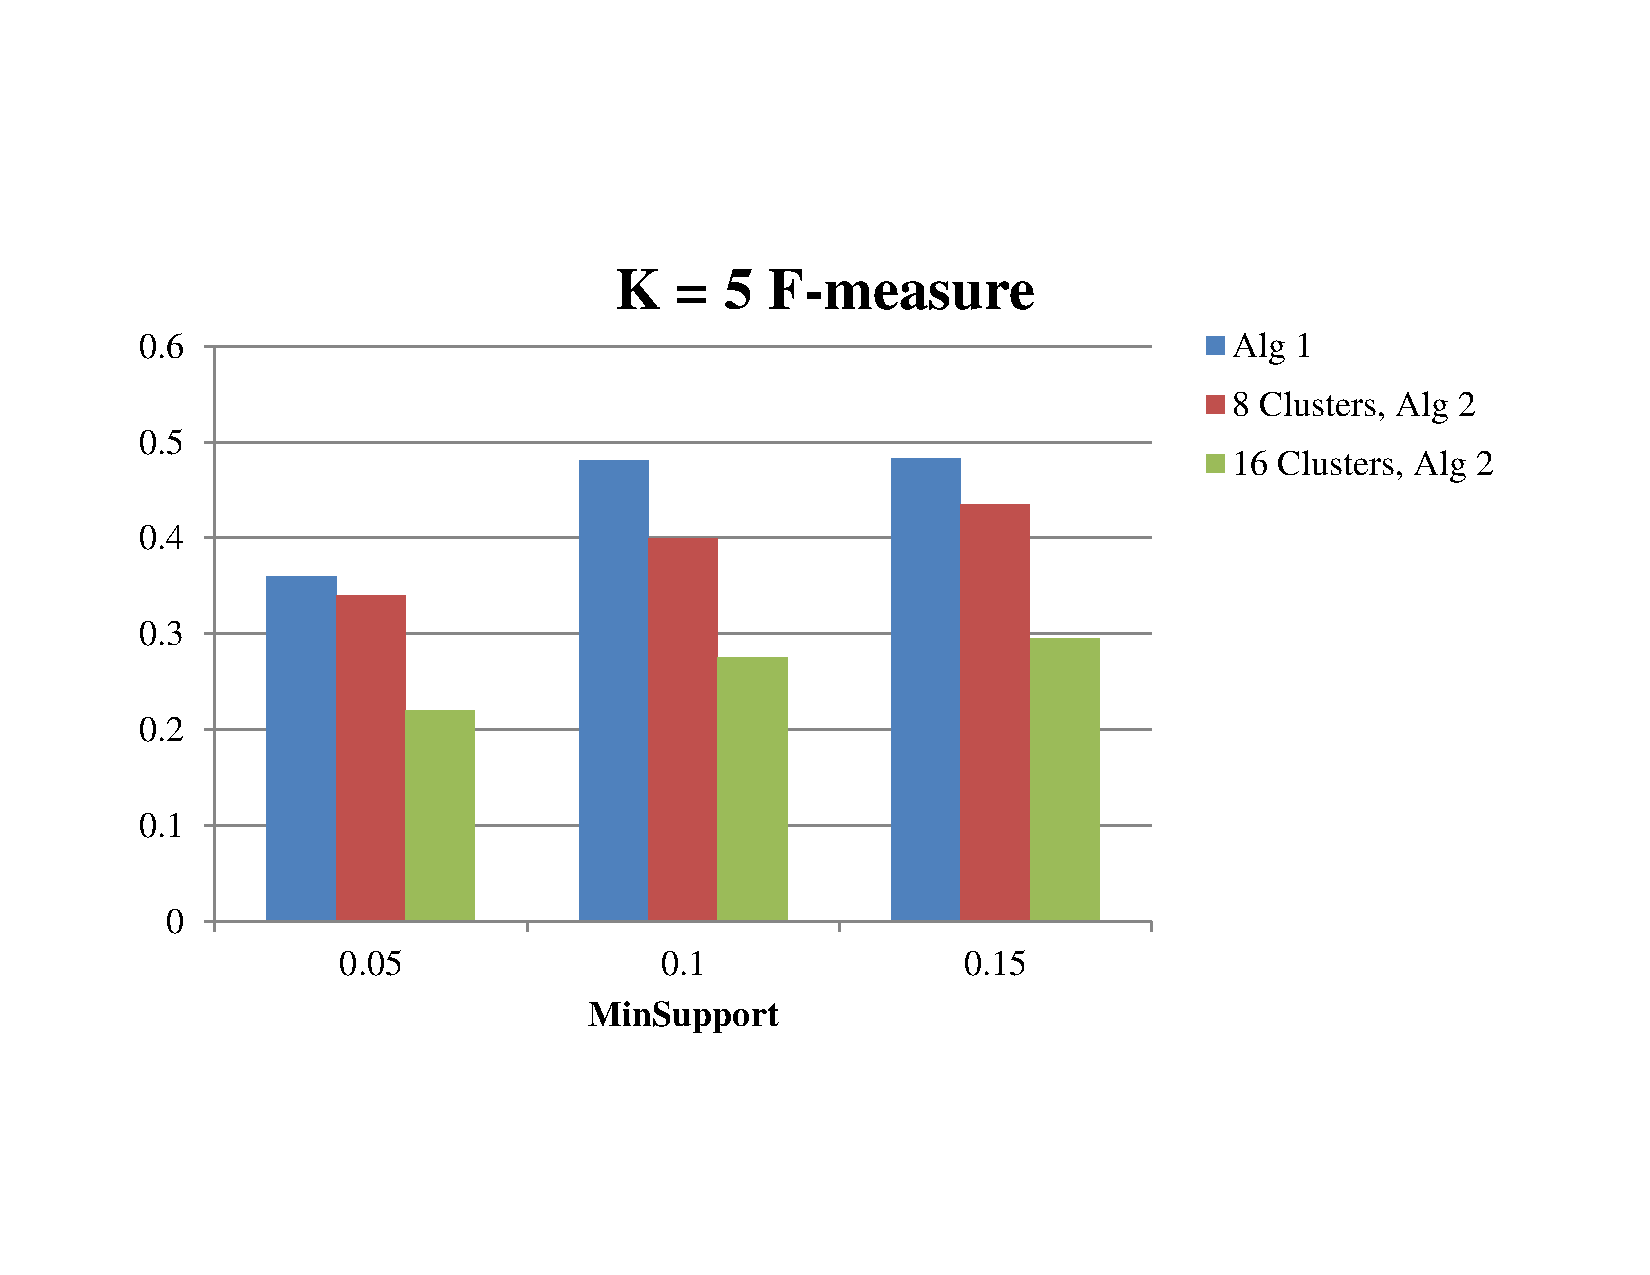
\includegraphics[width=\textwidth]{F-measure5}
         \caption{K = 5}
         \label{Fig:F-measure5}
        \end{subfigure}
        \caption{F-measures for two algorithms with different parameters.}
        \label{Fig:F-measure}
\end{figure*}
